\section*{\LARGE{Restauración del .backup}}

\section*{Introducción}

En esta sección, se detalla el proceso de restauración de una base de datos en un entorno de contenedores Docker utilizando PostgreSQL. Se utilizó el archivo de respaldo \texttt{transporte.backup} proporcionado por el ayudante para restaurar una base de datos de ejemplo. Este informe documenta los pasos seguidos para lograr una restauración exitosa, así como las evidencias que validan el proceso, \textit{(forma parte del punto IV de la entrega)}. \\

En escencia se siguieron los mismos pasos que se especifican en el documento de \textit{RestaurarBackupDocker.pdf} .

\section*{Pasos Realizados:} 


\subsection*{1. Verificación de Contenedores} 

Inicialmente verificamos los contenedores disponibles en Docker utilizando el comando: \\

\begin{verbatim}
    docker ps -a    
\end{verbatim}


\begin{figure}[h]
    \centering
        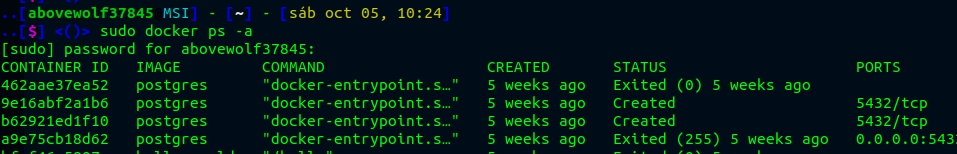
\includegraphics[width=1\textwidth]{../latex/resources/recovery/R1.png}
    \end{figure}

Despues de haber verificado los contenedores que había en el sistema, se procedió a obtener el ID de alguna de las imagenes de PostgreSQL que ya se encontraban creadas en el mismo. En este caso, se utilizó la imagen con ID \texttt{a9e75cb18d62} y procedimos a reiniciar el contenedor ya que había pasado mucho tiempo desde que se había creado. \\

\begin{figure}[h]
    \centering
        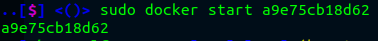
\includegraphics[width=1\textwidth]{../latex/resources/recovery/R2.png}
    \end{figure}

Checamos el estatus del contenedor con el comando \texttt{docker ps -a}. \\

\begin{figure}[h]
    \centering
        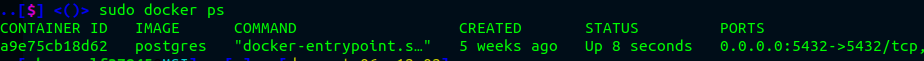
\includegraphics[width=1\textwidth]{../latex/resources/recovery/R3.png}
    \end{figure}

\subsection*{2. Conexión al Contenedor}

Una vez reiniciado el contenedor, procedimos a conectarnos a él utilizando el comando: \\

\begin{verbatim}
    sudo docker exec -it <CONTAINER_ID> psql -U postgres
\end{verbatim}

lo cual nos mete dentro de psql, una vez detro ejecutamos \textit{\l} donde podemos observar lo siguiente: \\

\begin{figure}[h]
    \centering
        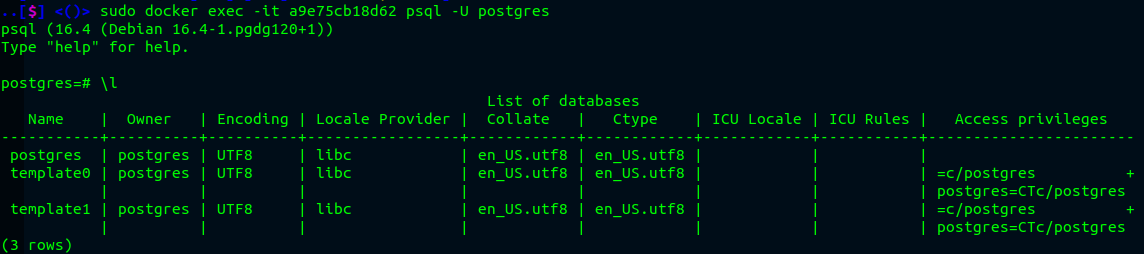
\includegraphics[width=1\textwidth]{../latex/resources/recovery/R4.png}
\end{figure}

salimos con \texttt{\textbackslash q}.

\subsection*{3. Restauración del .backup}

Como bien se menciona en el PDF, para hacer un backup necesitamos asegurarnos de que la base de datos esté vacía para evitar posibles conflictos con tablas repetidas. Entonces creamos una nueva base de datos a la cual llamaremos en esta ocasión \textit{transporte} con el ID del contenedor que hemos estado utilizando de la siguiente manera: \\

\begin{verbatim}
    sudo docker exec -it <CONTAINER_ID> createdb -U postgres ejemplo
\end{verbatim}

\begin{figure}[h!]
    \centering
        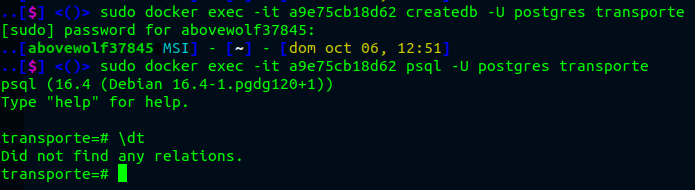
\includegraphics[width=1\textwidth]{../latex/resources/recovery/R5.png}
\end{figure}

Como se puede observar ejecutamos \textit{\textbackslash dt} para checar el contenido de la base de datos y vemos que efectivamente está vacía. De esta manera procedemos a la restauración del backup que en nuestro caso se encuentra en el archivo \textit{transporte.backup}. utilizamos el siguiente comando. \\

\begin{verbatim}
    sudo docker exec -i <CONTAINER_ID> pg_restore --verbose --clean --no-acl --no-owner -U 
    postgres -d transporte < /home/abovewolf37845/Downloads/backup/transporte.backup
\end{verbatim}

Notemos que en lugar de utilizar \textit{psql} utilizamos \textit{pg\_restore} ya que parece que \textit{psql} solamente para archivos sql y \textit{psql} para dump files. \\

\begin{figure}[h!]
    \centering
        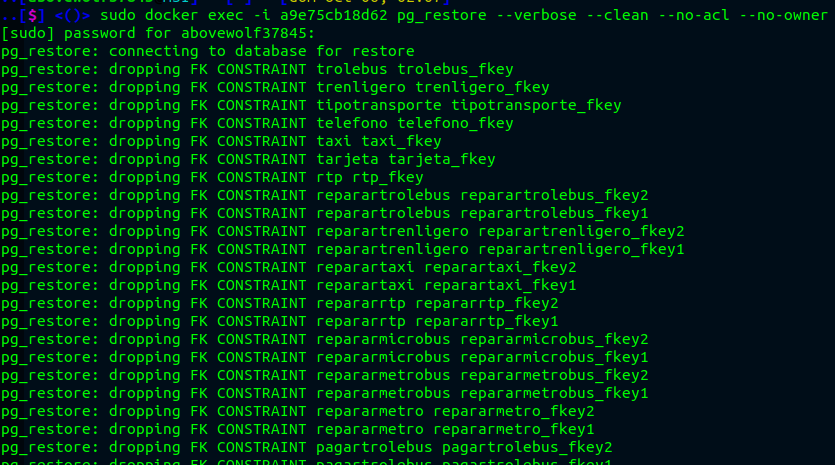
\includegraphics[width=1\textwidth]{../latex/resources/recovery/R6.png}
\end{figure}

\newpage

Después verificamos que la base de datos se haya restaurado correctamente con \textit{\textbackslash dt} dentro de psql donde veríamos algo como lo siguiente: \\ 

\begin{figure}[h!]
    \centering
        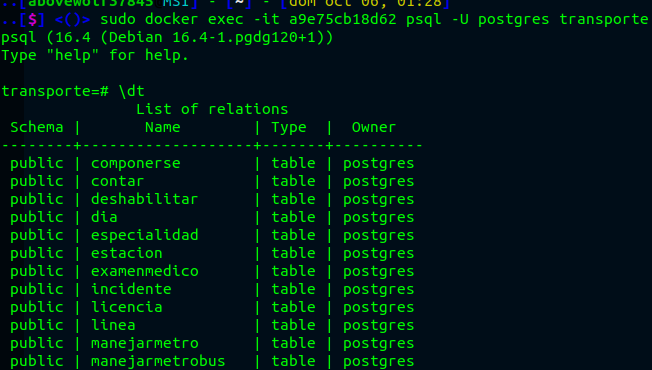
\includegraphics[width=1\textwidth]{../latex/resources/recovery/R7.png}
\end{figure}

Lo cual nos indica que restauramos la base de datos correctamente. \\

\subsection*{Para ver las bases de datos que se crearon en Dbeaver}

Seguimos las instrucciones para configurar correctamente el Database Tool DBeaver. \\

\begin{figure}[h!]
    \centering
        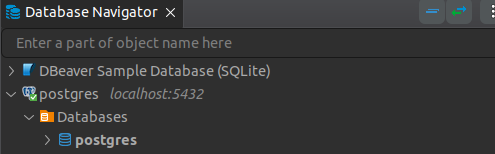
\includegraphics[width=1\textwidth]{../latex/resources/recovery/BD1.png}
\end{figure}

\begin{figure}[h!]
    \centering
        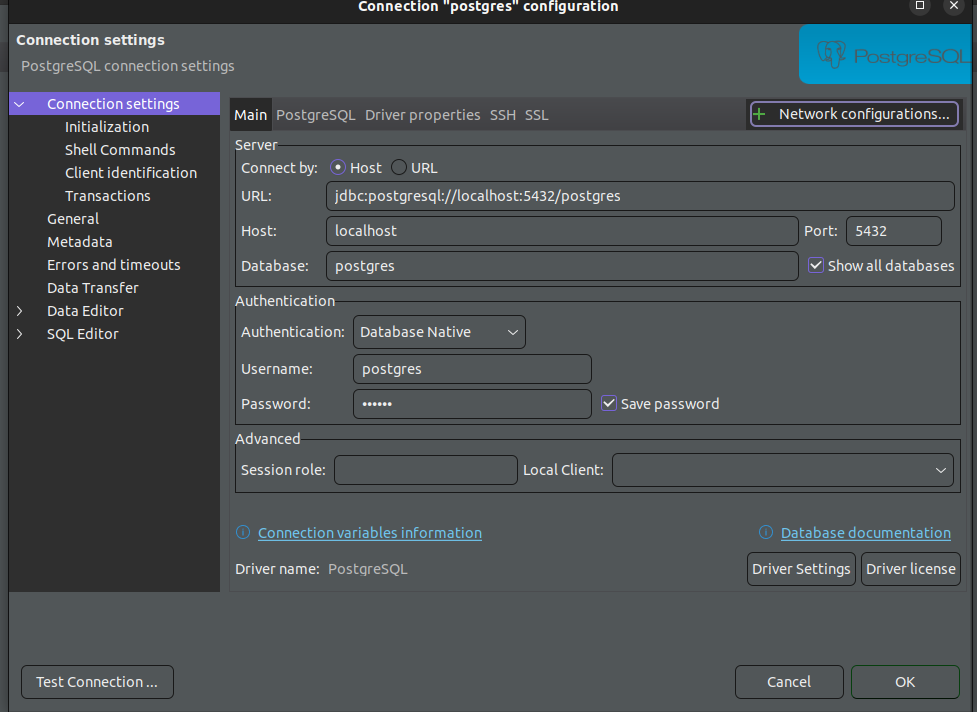
\includegraphics[width=1\textwidth]{../latex/resources/recovery/BD2.png}
\end{figure}

\begin{figure}
    \centering
        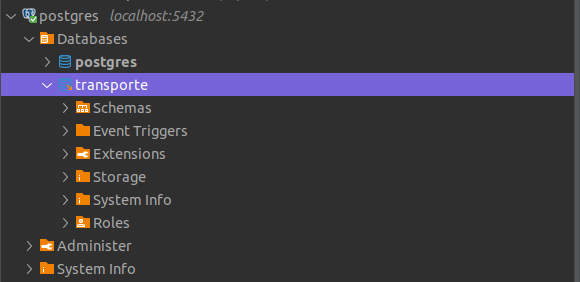
\includegraphics[width=1\textwidth]{../latex/resources/recovery/BD3.png}
\end{figure}

\newpage

Ahora podemos ver las bases de datos que se crearon en DBeaver. \\

\begin{figure}[h!]
    \centering
        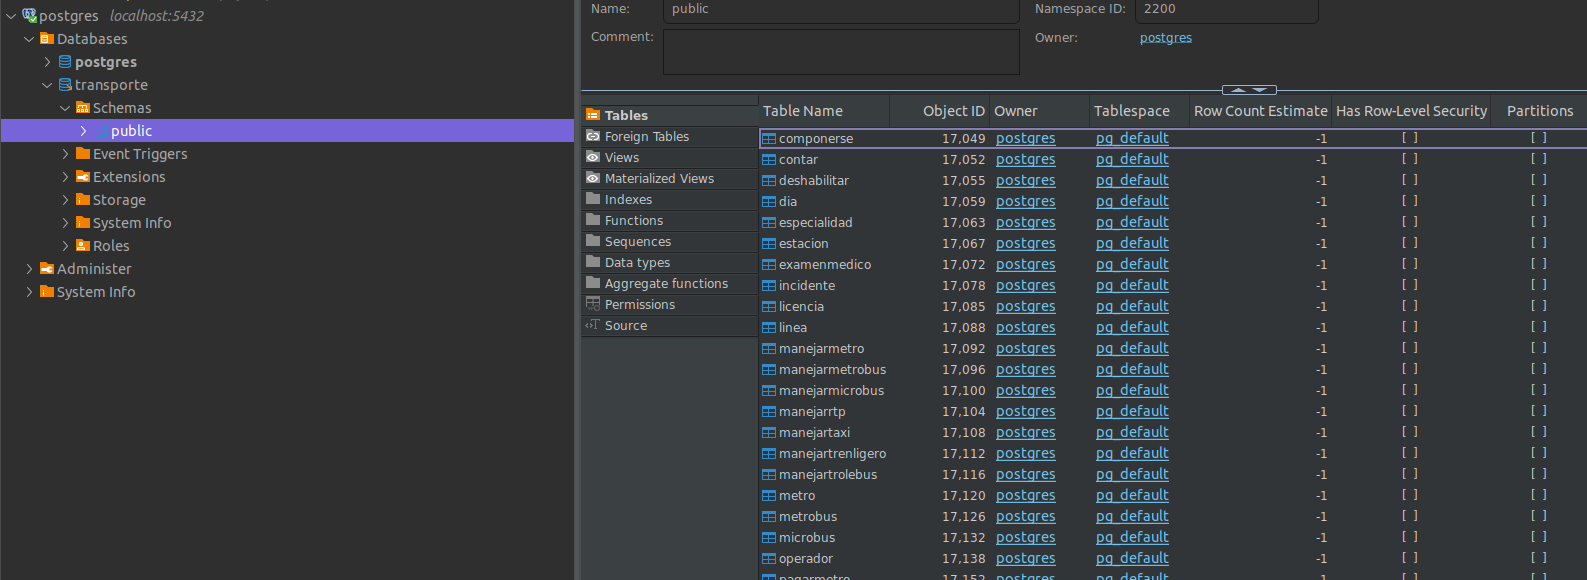
\includegraphics[width=1\textwidth]{../latex/resources/recovery/BD4.png}
\end{figure}